\documentclass[12pt]{article}
\usepackage{amsmath}
\usepackage{amssymb}
\usepackage[letterpaper,margin=0.85in,centering]{geometry}
\usepackage{fancyhdr}
\usepackage{enumerate}
\usepackage{lastpage}
\usepackage{multicol}
\usepackage{graphicx}

\reversemarginpar

\pagestyle{fancy}
\cfoot{Page \thepage \ of \pageref{LastPage}}\rfoot{{\bf Total Points: 50}}
\chead{MATH 1410A}\lhead{Test \# 1}\rhead{Monday, 3\textsuperscript{rd} October, 2016}

\newcommand{\points}[1]{\marginpar{\hspace{24pt}[#1]}}
\newcommand{\skipline}{\vspace{12pt}}
%\renewcommand{\headrulewidth}{0in}
\headheight 30pt

\newcommand{\di}{\displaystyle}
\newcommand{\R}{\mathbb{R}}
\newcommand{\aaa}{\mathbf{a}}
\newcommand{\bbb}{\mathbf{b}}
\newcommand{\ccc}{\mathbf{c}}
\newcommand{\dotp}{\boldsymbol{\cdot}}
\newcommand{\abs}[1]{\lvert #1\rvert}
\newcommand{\len}[1]{\lVert #1\rVert}
\newcommand{\ivec}{\,\boldsymbol{\hat{\imath}}}
\newcommand{\jvec}{\,\boldsymbol{\hat{\jmath}}}
\newcommand{\kvec}{\,\boldsymbol{\hat{k}}}
\newcommand{\bvm}{\begin{vmatrix}}
\newcommand{\evm}{\end{vmatrix}}

\DeclareMathOperator{\comp}{comp}

\begin{document}

\author{Instructor: Sean Fitzpatrick}
\thispagestyle{plain}
\begin{center}
\emph{University of Lethbridge}\\
Department of Mathematics and Computer Science\\
3\textsuperscript{rd} October, 2016, 9:00 - 9:50 am\\
{\bf MATH 1410A - Test \#1}\\
\end{center}
\skipline \skipline \skipline \noindent \skipline
Last Name:\underline{\hspace{353pt}}\\
\skipline
First Name:\underline{\hspace{350pt}}\\
\skipline
Student Number:\underline{\hspace{323pt}}\\
\skipline
Tutorial Section: \underline{\hspace{320pt}}\\


\vspace{0.5in}


\begin{quote}
 {\bf Record your answers below each question in the space provided.    Left-hand pages may be used as scrap paper for rough work.  If you want any work on the left-hand pages to be graded, please indicate so on the right-hand page.
 
 \bigskip
 
Partial credit will be awarded for partially correct work, including intermediate steps. (You should show your work if you want to earn part marks.) Unless otherwise indicated, failure to justify your work may result in loss of marks, even for a correct answer. 

\bigskip

No external aids are allowed, with the exception of a 5-function calculator.}
\end{quote}


\vspace{0.5in}

For grader's use only:

\begin{table}[hbt]
\begin{center}
\begin{tabular}{|l|r|} \hline
Page&Grade\\
\hline \hline
\cline{1-2} 2 & \enspace\enspace\enspace\enspace\enspace\enspace/14\\
\cline{1-2} 3 & \enspace\enspace\enspace\enspace\enspace\enspace/14\\
\cline{1-2} 4 & \enspace\enspace\enspace\enspace\enspace\enspace/12\\
\cline{1-2} 5 & \enspace\enspace\enspace\enspace\enspace\enspace/10\\
\cline{1-2} Total & \enspace\enspace\enspace\enspace\enspace\enspace/50\\
\hline
\end{tabular}

\skipline

\skipline

\skipline

B
\end{center}
\end{table}
\newpage


\begin{enumerate}
\item Given the complex numbers $z=1+3i$ and $w=2-2i$, compute the following. You do not need to explain your work.
 \begin{enumerate}
\item $z+w$ \points{2}

\[
 z+w = (1+3i)+(2-2i) = (1+2)+i(3-2) = 3+i.
\]

\bigskip

\item $\overline{z}$ \points{2}

Using the formula $\overline{x+iy} = x-iy$,

\[
 \overline{z} = \overline{1+3i} = 1-3i.
\]

\bigskip

\item $\abs{w}$ \points{2}

Using the formula $\abs{a+ib} = \sqrt{a^2+b^2}$,

\[
 \abs{w} = \abs{2-2i} = \sqrt{2^2+(-2)^2} = \sqrt{4+4}=\sqrt{8}.
\]

\bigskip

\item $zw$ \points{2}

\[
 zw = (1+3i)(2-2i) = 1(2)+1(-2i)+3i(2)+3i(-2i) = 2-2i+6i-6i^2 = 2+4i-6(-1) = 8+4i.
\]

\bigskip

\item $\dfrac{z}{w}$ \points{3}

\[
\frac{z}{w} = \frac{1+3i}{2-2i} = \frac{(1+3i)(2+2i)}{(2-2i)(2+2i)} = \frac{2-6+i(2+6)}{4+4} = \frac{-4+8i}{8} = -\frac{1}{2}+i. 
\]


\item The polar form of $w$. \points{3}

\[
 2-2i = 4\left(\frac{1}{2}+i\left(-\frac{1}{2}\right)\right) = 4\left(\cos\left(-\frac{\pi}{4}\right)+i\sin\left(-\frac{\pi}{4}\right)\right) = 4e^{-i\pi/4}.
\]

\end{enumerate}

\newpage

\item Given the vectors $\vec{v} = \langle 0, 3, -2\rangle$ and $\vec{w} = \langle -1, 1, 4\rangle$, compute the following. You do not need to explain your work.
\begin{enumerate}
 \item $\vec{v}-3\vec{w}$  \points{2}

\[
 \vec{v}-3\vec{w} = \langle 0,3,-2\rangle-3\langle -1,1,4\rangle = \langle 0,3,-2\rangle+\langle 3,-3,-12\rangle = \langle 3,0,-14\rangle.
\]

  
 \item $\len{\vec{v}}$ \points{2}

\[
 \len{\vec{v}} = \sqrt{0^2+3^2+(-2)^2} = \sqrt{9+4}=\sqrt{13}.
\]


 \item $\vec{v}\dotp\vec{w}$ \points{2}

\[
 \vec{v}\dotp\vec{w}=\langle 0,3,-2\rangle\dotp \langle -1,1,4\rangle = 0(-1)+3(1)-2(4) = 0+3-8=-5.
\]


 \item $\vec{v}\times \vec{w}$ \points{4}

\begin{align*}
 \vec{v}\times\vec{w} &= \begin{vmatrix}
                         \hat{\imath} & \hat{\jmath} & \hat{k}\\
			 0&3&-2\\-1&1&4
                        \end{vmatrix} = \hat{\imath}(3(4)-(-2)(1))-\hat{\jmath}(0(4)-(-2)(-1))+\hat{k}(0(1)-3(-1))\\
& = 14\hat{\imath}+2\hat{\jmath}+3\hat{k} = \langle 14,2,3\rangle.
\end{align*}

 \item $\operatorname{proj}_{\vec{v}}\vec{w}$ \points{4}

Using the values $\vec{v}\dotp\vec{w} = -5$ and $\len{\vec{v}} = \sqrt{13}$ from above, we have
\[
 \operatorname{proj}_{\vec{v}}\vec{w} = \left(\frac{\vec{v}\dotp\vec{w}}{\len{\vec{v}}^2}\right)\vec{v} = \frac{-5}{13}\langle 0,3,-2\rangle = \left\langle 0,-\frac{15}{13},\frac{10}{13}\right\rangle.
\]
\end{enumerate}
\newpage

\item 
\begin{enumerate}
 \item Verify that $z=-\sqrt{2}-i\sqrt{2}$ can be written in the polar form $z=2e^{i(5\pi/4)}$. \points{3}

This is most easily verified by checking that the given polar form reduces to the correct complex number. Using Euler's formula, we have
\[
 2e^{i(5\pi/4)} = 2\left(\cos\frac{5\pi}{4}+i\sin\frac{5\pi}{4}\right) = 2\left(-\frac{\sqrt{2}}{2}-i\frac{\sqrt{2}}{2}\right) = -\sqrt{2}-i\sqrt{2},
\]
as required.

If we instead begin with the rectangular form, we must first compute \\$\abs{z} = \sqrt{(-\sqrt{2})^2+(-\sqrt{2})^2} = \sqrt{2+2}=2$, and then note that
\[
 -\sqrt{2}-i\sqrt{2} = 2\left(-\frac{\sqrt{2}}{2}-i\frac{\sqrt{2}}{2}\right).
\]
From here, we can use the given unit circle to look up the angle $\theta$ for which $\cos\theta = -\frac{\sqrt{2}}{2}$ and $\sin\theta = -\frac{\sqrt{2}}{2}$.

For full marks, it needed to be clear from your solution that you understood that the correct angle was determined from the fact that $x<0$ and $y>0$ in the second quadrant, and not simply because you knew what the answer was supposed to be.
\medskip

 \item Compute the power $(-\sqrt{2}-i\sqrt{2})^5$. Express your answer in the form $x+iy$. \points{5}
\end{enumerate}

\bigskip

From part (a), we have
\[
 (-\sqrt{2}-i\sqrt{2})^5 = \left(2e^{i(5\pi/4)}\right)^5 = 2^5\left(e^{i(5\pi/4)}\right)^5 = 2^5e^{i(25\pi/4)}.
\]
Since $\dfrac{25\pi}{4} = \dfrac{24\pi}{4}+\dfrac{\pi}{4} = 6\pi+\dfrac{\pi}{4}$, we have
\[
 2^5e^{i(25\pi/4)} = 32e^{i\pi/4} = 32\left(\cos \frac{\pi}{4}+i\sin\frac{\pi}{4}\right) = 32\left(\frac{\sqrt{2}}{2}+i\frac{\sqrt{2}}{2}\right) = 16\sqrt{2}+16\sqrt{2}i.
\]



\item Find the point of intersection of the line $\langle x,y,z\rangle = \langle 4, -1, 3\rangle+t\langle 2, 0, -1\rangle$ and the plane $x+3y-2z=3$. \points{4}

\bigskip

Let $(x,y,z)$ denote the point of intersection. Since $(x,y,z)$ lies on the line, we know from the equation of the line that
\[
 \langle x,y,z\rangle = \langle 4+2t,-1,3-t\rangle,
\]
so $x=4+2t$, $y=-1$, and $z=3-t$. Substituting these values into the equation of the plane (which the point $(x,y,z)$ must also satisfy), we have
\begin{align*}
 (4+2t)+3(-1)-2(3-t) & = 3\\
 4+2t-3-6+2t&=3\\
 4t-5&=3\\
 4t & = 8\\
 t&=2.
\end{align*}

Putting $t=2$ into the parametric equations of the line given above, we have $x=4+2(2)=8$, $y=-1$, and $z=3-(2) = 1$, so our point of intersection is $(8,-1,1)$.
\newpage

\item Find the vector equation of the line $\ell$ that passes through the points $P=(0, 3, -2)$ and $Q=(1, 4, -1)$. \points{4}

\bigskip

To obtain the equation of a line in $\R^3$, we need a point on the line, and a direction vector. Choosing $P=(0,3,-2)$ as our point on the line, it remains to determine a direction vector. Since $P$ and $Q$ are both on the line, the vector
\[
 \vec{v} = \overrightarrow{PQ} = \langle 1-0, 4-3, -1-(-2)\rangle = \langle 1,1,1\rangle
\]
is in the direction of the line, and thus, we can write the vector equation of our line as
\[
 \langle x,y,z\rangle = \langle 0,3,-2\rangle + t\langle 1,1,1\rangle.
\]


Compute \textbf{one} of the following two distances. \points{6} To earn full marks, your solution must include a clearly labelled diagram.
\begin{itemize}
\item From the point $P=(4, 5, 2)$ to the line $\langle x,y,z\rangle = \langle 2,1,-1\rangle + t\langle 0,1,2 \rangle$ 

\medskip

\begin{multicols}{2}
 \begin{center}
  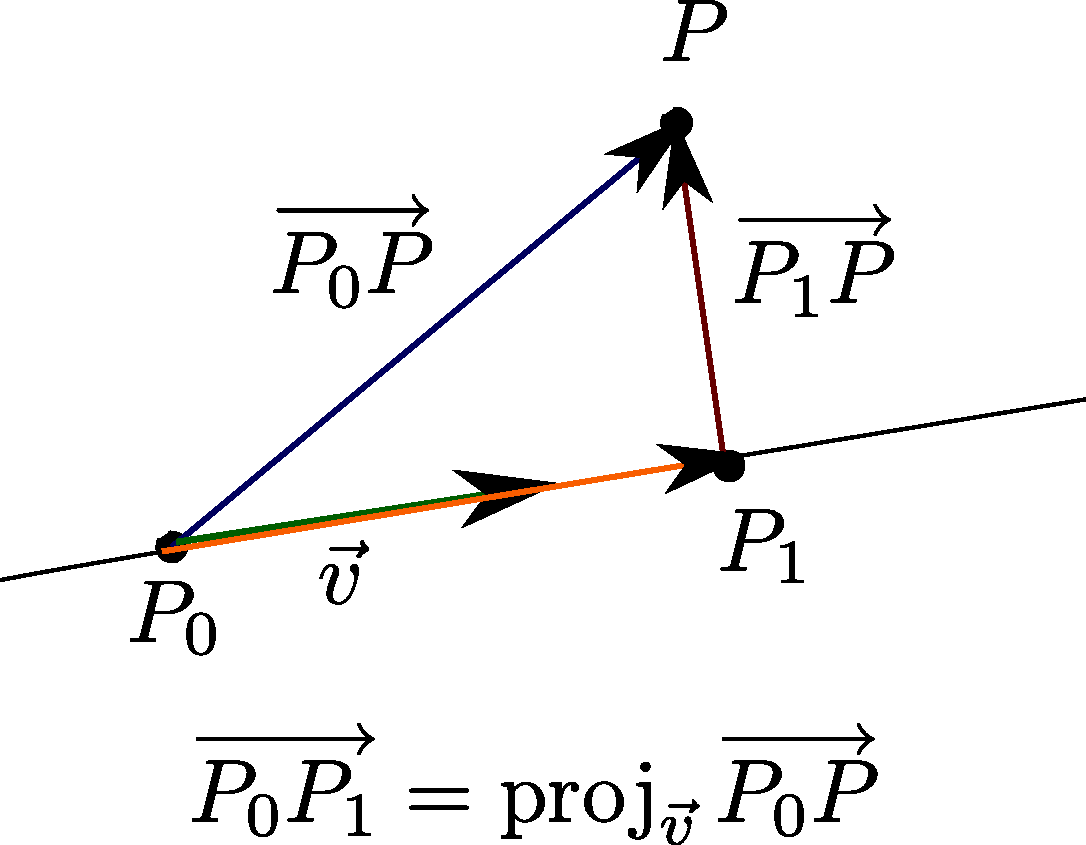
\includegraphics[width=0.75\columnwidth]{WS3-3}
 \end{center}
\columnbreak

Referring to the diagram to the left, we have $P=(4,5,2)$, and we can choose $P_0 = (2,1,-1)$ as a point on our line, giving us the vector
\[
 \vec{w} = \overrightarrow{P_0P} = \langle 2,4,3\rangle.
\]
From the equation of the line, we have the direction vector $\vec{v} = \langle 0,1,2\rangle$. Again, referring to the diagram, we can see that the vector $\overrightarrow{P_0P_1}$ is given by the projection of $\vec{w}$ onto $\vec{v}$. We compute:
\end{multicols}
\[
 \overrightarrow{P_0P_1} = \left(\frac{\vec{v}\dotp\vec{w}}{\len{\vec{v}}^2}\right)\vec{v} = \frac{10}{5}\langle 0,1,2\rangle = \langle 0,2,4\rangle.
\]
The desired distance is given by the length of the vector $\overrightarrow{P_1P}$. From the diagram, we have
\[
 \overrightarrow{P_1P} = \overrightarrow{P_0P}-\overrightarrow{P_0P_1} = \langle 2,4,3\rangle - \langle 0,2,4\rangle = \langle 2,2,-1\rangle.
\]
The distance is therefore $d=\len{\overrightarrow{P_1}} = \sqrt{2^2+2^2+(-1)^2} = \sqrt{9}=3$.

\newpage

\item From the point $P=(2,5,8)$ to the plane $2x-3y+z=4$.

\begin{multicols}{2}
 \begin{center}
  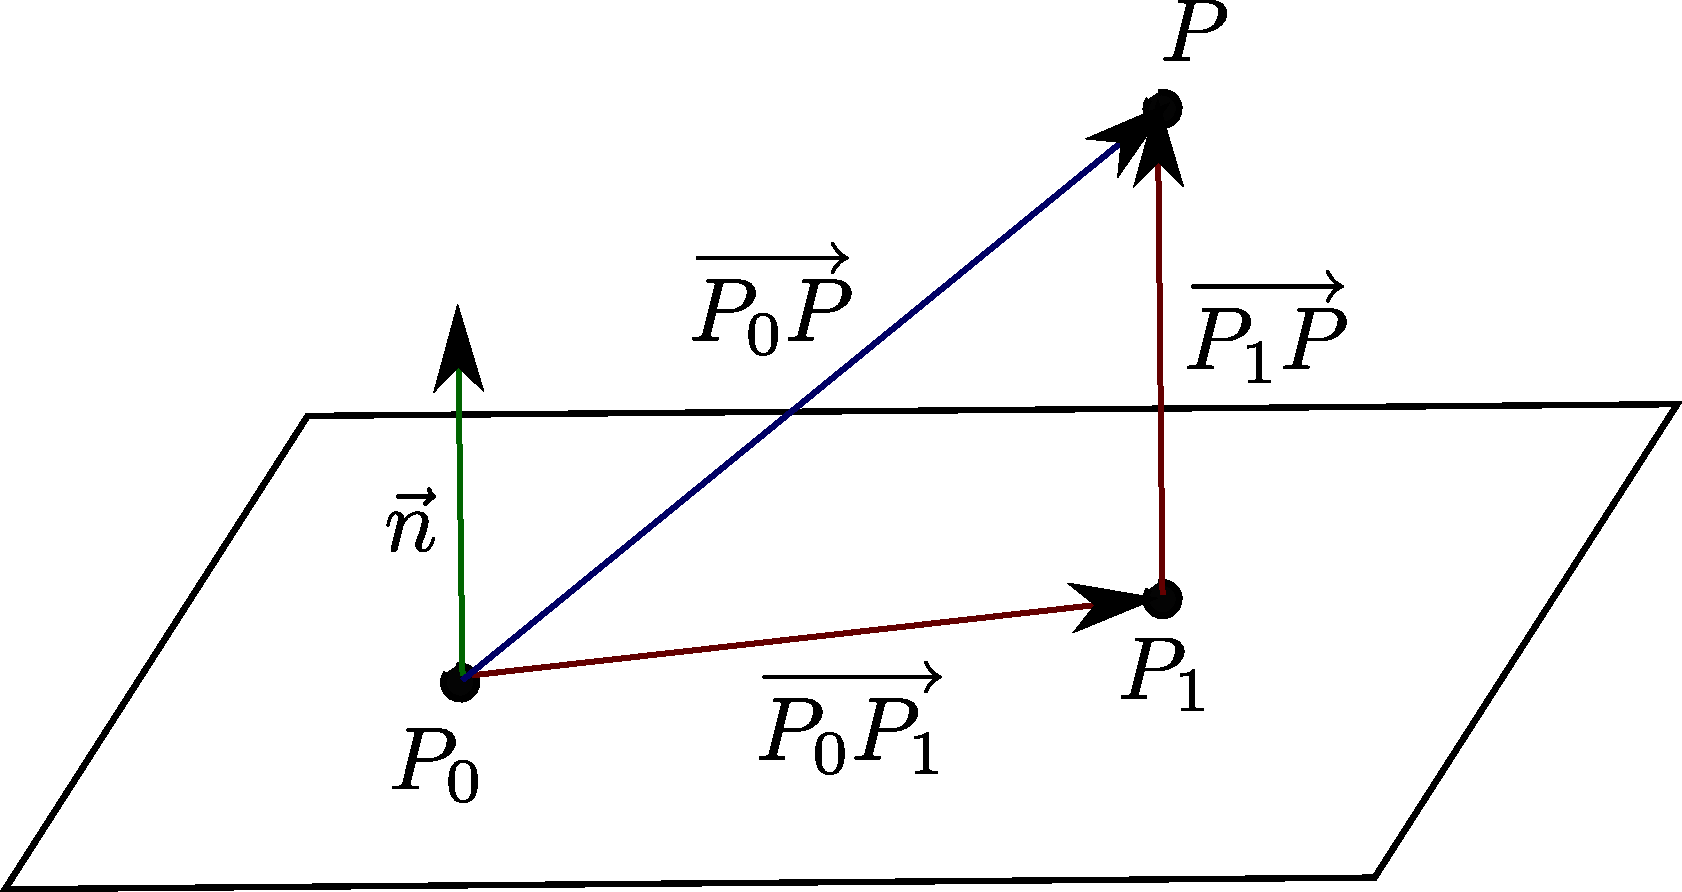
\includegraphics[width=0.75\columnwidth]{WS3-4}
 \end{center}
\columnbreak

To obtain the point $P_0$ in our diagram to the left, we choose any point on the plane. One possibility (of many) is the point $(0,0,4)$, since $2(0)-3(0)+4=4$. We're given $P=(2,5,8)$, from which we obtain the vector 
\[
 \vec{w} = \overrightarrow{P_0P} = \langle 2-0,5-0,8-4\rangle = \langle 2,5,4\rangle.
\]
From the equation of the plane we have the normal vector $\vec{n} = \langle 2,-3,1\rangle$. 
\end{multicols}
The desired distance is given by the magnitude of the vector $\overrightarrow{P_1P}$; from the diagram, we have
\[
 \overrightarrow{P_1P} = \operatorname{proj}_{\vec{n}}\vec{w}.
\]
The distance is therefore equal to
\[
 \left\lVert\left(\frac{\vec{w}\dotp\vec{n}}{\len{\vec{n}}^2}\right)\vec{n}\right\rVert = \frac{\abs{\vec{w}\dotp\vec{n}}}{\len{\vec{n}}} = \frac{\abs{4-15+4}}{\sqrt{2^2+(-3)^2+1^2}} = \frac{7}{\sqrt{14}}.
\]
\end{itemize}




\end{enumerate}
\end{document}